\subsection{Parallel Combinations of FREEs}
\label{sec:parallelActuators}
We can extend the concept of a fluid Jacobian to systems with multiple actuators that are mounted in parallel.
FREEs that are mounted in parallel each have one end attached to a common ground and the other rigidly attached to an end effector.
The position and orientation of this end effector is given by a deformation vector $\vec{x}$, and we assume that an inverse kinematics function allows the computation of the state $\vec{q}_i \left(\vec{x}\right)$ for each individual FREE.
To express forces and torques in a common reference frame, we define a body-fixed reference point and coordinate system that are attached to the end effector (Fig.~\ref{fig:dp_defined}). 
Expressed in these coordinates, a position vector ${\vec{d}_i = \begin{bmatrix} d_i^{\hat{x}_e} & d_i^{\hat{y}_e} & d_i^{\hat{z}_e} \end{bmatrix}^T}$ defines the point where the $i$th FREE is attached, and a unit vector ${\hat{a}_i = \begin{bmatrix} a_i^{\hat{x}_e} & a_i^{\hat{y}_e} & a_i^{\hat{z}_e} \end{bmatrix}^T}$, expresses the direction of the associated FREE axis.

Let $\vec{f}_i$ be the vector of general forces exerted by the $i$th FREE and expressed in end effector coordinates:
\begin{align}
    \vec{f}_i = \bmx F^{\hat{x}_e}_i & F^{\hat{y}_e}_i & F^{\hat{z}_e}_i & M^{\hat{x}_e}_i & M^{\hat{y}_e}_i & M^{\hat{z}_e}_i \emx^T,
\end{align}
where $F^{\hat{x}_e}_i$ is the component of force along the $x$-axis of the end effector frame and $M^{\hat{x}_e}_i$ is the moment about the $x$-axis of that frame.
The components of this vector can be computed from the axial force $F_i$ and twisting torque $M_i$ of the $i$th FREE as:
\begin{align}
    \bmx F^{\hat{x}_e}_i & F^{\hat{y}_e}_i & F^{\hat{z}_e}_i \emx^T &= \hat{a}_i F_i ,   \label{eq:Df}
\end{align}
and
\begin{align}
    \bmx M^{\hat{x}_e}_i & M^{\hat{y}_e}_i & M^{\hat{z}_e}_i \emx^T &= \lfloor \vec{d}_i \times \rfloor \hat{a}_i F_i + \hat{a}_i M_i,    \label{eq:Dm}
\end{align}
where $\lfloor \vec{d}_i \times \rfloor$ is the matrix notation for the cross-product with $\vec{d}_i$:
\begin{align}
    \lfloor \vec{d}_i \times \rfloor &= \begin{bmatrix} 0 & -d_i^{\hat{z}_e} & d_i^{\hat{y}_e} \\ d_i^{\hat{z}_e} & 0 & -d_i^{\hat{x}_e} \\ -d_i^{\hat{y}_e} & d_i^{\hat{x}_e} & 0 \end{bmatrix}. 
\end{align}
Combining \eqref{eq:Df} and \eqref{eq:Dm} into a single transformation yields:
\begin{align}
    \vec{f}_i &= \bar{\mathcal{D}}_i \vec{\tau}_i,  \label{eq:zetai}
\end{align}
where $\mathcal{D}_{i}$ is the $6 \times 2$ matrix:
\begin{align}
    \bar{\mathcal{D}}_i &= \begin{bmatrix}
                    \begin{bmatrix} \hat{a}_i & \vec{0}_{3\times1} \end{bmatrix} \vspace{5pt} \\ 
                    \begin{bmatrix} \lfloor \vec{d}_i \times \rfloor \hat{a}_i & \vec{0}_{3\times1} \end{bmatrix} + \begin{bmatrix} \vec{0}_{3\times1} & \hat{a}_i \end{bmatrix}
                    \end{bmatrix}.   \label{eq:D}
\end{align}


\begin{figure}
    \centering
    \begin{tikzpicture}
        \node (diagram) at (0,0)
            {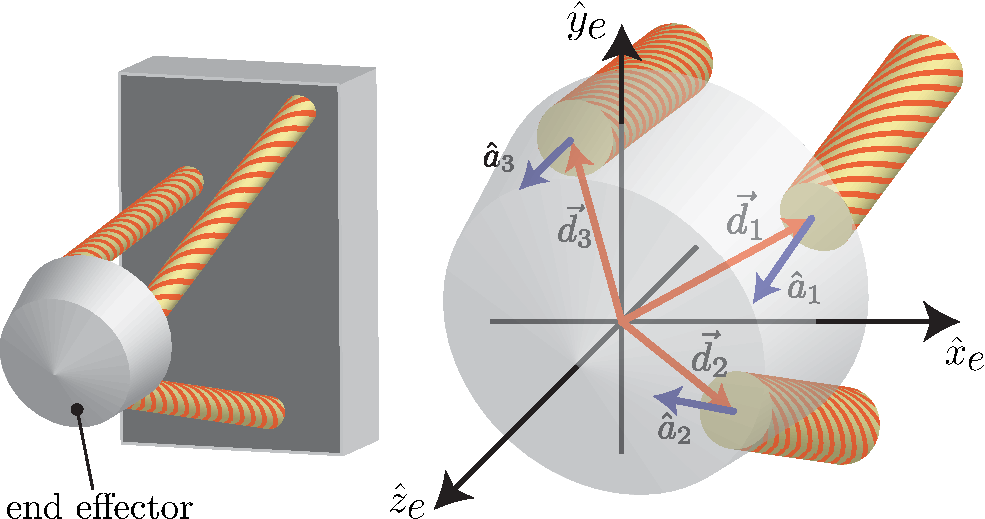
\includegraphics[width=1.0\linewidth]{figures/dp_defined-revised-v2.pdf}};
        \node[below] (a) at ($ (diagram.south west) !0.22! (diagram.south east) $) {(a)};
        \node[below] (b) at ($ (diagram.south west) !0.65! (diagram.south east) $) {(b)};
    \end{tikzpicture}
%    (a) An arbitrary combination of 3 FREEs connected to a common end effector. (b) A zoomed in view of the end effector with its local coordinate frame shown.}
    \caption{\revcomment{2.7}{(a) When multiple FREEs are attached in parallel to the same end effector, shown on the left, we must consider their relative positions and orientations. (b) This is determined by the vector $\vec{d}_i$ of the displacement of the attachment point of a FREE relative to the origin of the end effector frame, and by the unit vector $\hat{a}_i$ that is aligned with the FREE axis at the attachment point, shown in the zoomed-in view on the right.}}
    \label{fig:dp_defined}
\end{figure}


Since the actuators are mounted in parallel, the total force $\vec{f}$ is the sum of the individual forces of all $n$ FREEs connected to the end effector: 
\begin{align}
    \vec{f}(\vec{q}, \vec{p}) &= \sum_{i=1}^n \vec{f}_{i} = \sum_{i=1}^n \bar{\mathcal{D}}_i \bar{J}^T_{q, i} (\vec{q}_i) p_i = \sum_{i=1}^n \bar{J}^T_{x, i} (\vec{x}) p_i,
    \label{eq:zeta}
\end{align}
where $\bar{J}_{x, i} = \bar{J}_{q, i} \bar{\mathcal{D}}^T_i$ is the fluid Jacobian of an individual FREE expressed in end effector coordinates and the vector $\vec{p}$ contains the internal pressure values of all FREEs.

This can be written compactly in matrix notation as 
\begin{align}
    \vec{f} (\vec{x}, \vec{p}) &= \bar{J}^T_x (\vec{x}) \vec{p}, \label{DAVIDreallyLIKESthisEQUATION}
\end{align}
with the overall fluid Jacobian $\bar{J}_x$:
\begin{align}
    \bar{J}_x &= \bmx \bar{J}^T_{x, 1} & \bar{J}^T_{x, 2} & \cdots & \bar{J}^T_{x, n} \emx^T
\end{align}

\subsection{The Force Zonotope}
Equation \eqref{DAVIDreallyLIKESthisEQUATION} shows that the force capability of the parallel combination of multiple FREEs is a linear function of the pressures in the individual actuators.
Since the fluid Jacobian $\bar{J}_{x}$ depends on the end effector state $\vec{x}$, the ability of such a system to generate forces at the end effector will vary based on its displacement.
For some values of $\vec{x}$ it may be possible to generate spacial forces in multiple directions, while for others the span of possible forces may by narrower. 
The \emph{force zonotope} of a parallel combination of FREEs, similar to the force ellipsoid of rigid manipulators, 
% \cite{spong2008robot}
describes the set of forces that can be generated at the end effector with a bounded set of input pressures.

\begin{definition}[Force Zonotope]
    For a parallel combination of $n$ FREEs, the force zonotope is the set of active general 
%    torques and
    forces that can be generated in a specific end effector state, $\vec{x}$,
    \begin{align}
        \mathcal{Z}(\vec{x}) &= \left\{\bar{J}^T_x (\vec{x}) \vec{p} \, : \, p_i \in [0,p_i^\text{max}] \right\}     \label{eq:zonotope}
    \end{align}
    where $p_i^{\text{max}}$ is the maximum pressure allowed for the $i^{th}$ FREE.
\end{definition}

Note that the \emph{force zonotope} is the convex hull of all spacial forces generated when $p_i \in \{0, p_i^{\text{max}}\}$.
This makes it viable to compute using a convex hull algorithm. By calculating the zonotope over a range of states, it can be used to verify that a given parallel FREE design is capable of generating the desired forces over the range of its workspace. 
%In this way, the \emph{force zonotope} provides insight into how to utilize FREEs as actuators for robotic systems.


To illustrate the design utility of the force zonotope, consider the parallel combination of FREEs shown in Figure~\ref{fig:zntpConstructed}.
Here, pairs of FREEs with opposite chirality are connected to the two sides of an end effector.
This end effector is constrained to slide and rotate exclusively along and about its $z$-axis.
Since the motion of the end-effector is two-dimensional, we would like to achieve controllable forces within these two dimensions; that is, have control authority over $F^{\vec{z}_e}$ and $M^{\vec{z}_e}$.
When constructing the zonotope one FREE at time (Figure~\ref{fig:zntpConstructed}a-d), one can observe how all four FREEs are needed to achieve this control authority.
In particular, it becomes evident that to achieve full control in $n$ dimensions, at least $n+1$ individual FREEs are required in an antagonistic configuration.
The additional FREE is needed since these soft actuators cannot be driven with negative pressure and can hence not produce bidirectional forces.
One can also observe that if the FREEs are chosen or arranged poorly such that the directions in $\bar{J}_{x}$ do not cover the space of desired forces (such as in Fig.~\ref{fig:zntpConstructed}c), this minimum number of actuators might not be sufficient.

\begin{figure}
    \centering

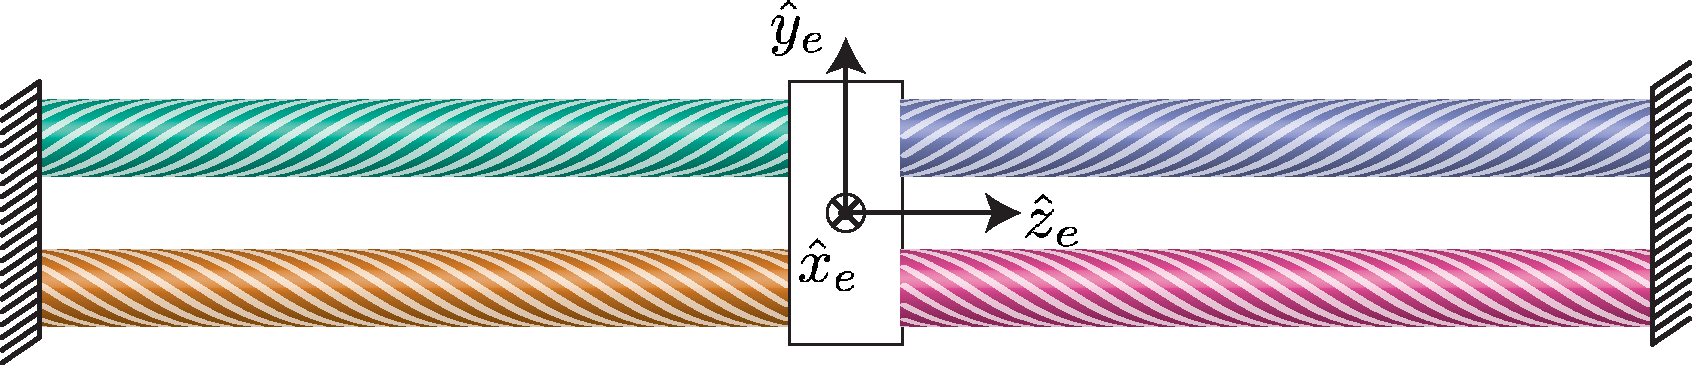
\includegraphics[width=0.85\linewidth]{figures/zntpExampleRig3.pdf}

\begin{tikzpicture}
\def\scl{0.45} % define scale variable for plots

% PRACTICE PLOT
\matrix [row sep=0.25cm, column sep=0cm, style={align=center}] (my matrix) at (0,0)
{

\begin{axis}[
    view={90}{0},
    axis lines=center,
    % axis equal image,
    xlabel={$M^{\hat{x}_e}$},
    ylabel={$F^{\hat{z}_e}$},
    zlabel={$M^{\hat{z}_e}$},
    ymin=-7, ymax=7, ytick={0}, %ylabel near ticks,
    xmin=-5, xmax=10, xtick={0}, %xticklabel=$\pgfmathprintnumber{\tick}^\circ$, xlabel near ticks, 
    zmin=-7, zmax=7, ztick={0}, %z dir=reverse,
    xlabel style={anchor=north}, ylabel style={anchor=north},
    scale=\scl,
    anchor=center,
    name=plot1,
    ]
    \def\pa{(-2,-3,2)}
    \def\pb{(2,-3,-2)}
    \def\pc{(2,3,-2)}
    \def\pd{(-2,3,2)}
    \addplot3[->, line width=1pt, plgreen] coordinates {(0,0,0) \pa};
%    \addplot3[->, line width=1pt, plorange] coordinates {(0,0,0) \pb};
%    \addplot3[->, line width=1pt, plpurple] coordinates {(0,0,0) \pc};
%    \addplot3[->, line width=1pt, plpink] coordinates {(0,0,0) \pd};
    % connector lines for perspective
    \addplot3[dotted] coordinates {(0,0,0) (-2,-3,0)};
    \addplot3[dotted] coordinates {(-2,-3,0) \pa}; 
%    \addplot3[dotted] coordinates {(0,0,0) (2,-3,0)};
%    \addplot3[dotted] coordinates {(2,-3,0) \pb};
%    \addplot3[dotted] coordinates {(0,0,0) (2,3,0)};
%    \addplot3[dotted] coordinates {(2,3,0) \pc};
%    \addplot3[dotted] coordinates {(0,0,0) (-2,3,0)};
%    \addplot3[dotted] coordinates {(-2,3,0) \pd};
    % faces of shape
%    \addplot3[patch, opacity=0.3, fill=black!20, faceted color=black, patch type=rectangle] 
%        coordinates {
%                    (0,0,0) \pa (0,-6,0) \pb
%                    (0,0,0) \pb (4,0,-4) \pc
%                    (0,0,0) \pc (0,6,0) \pd
%                    (0,0,0) \pd (-4,0,4) \pa
%                    };
\end{axis};

&

\begin{axis}[
    view={90}{0},
    axis lines=center,
    % axis equal image,
    xlabel={$M^{\hat{x}_e}$},
    ylabel={$F^{\hat{z}_e}$},
    zlabel={$M^{\hat{z}_e}$},
    ymin=-7, ymax=7, ytick={0}, %ylabel near ticks,
    xmin=-5, xmax=10, xtick={0}, %xticklabel=$\pgfmathprintnumber{\tick}^\circ$, xlabel near ticks, 
    zmin=-7, zmax=7, ztick={0}, %z dir=reverse,
    xlabel style={anchor=north}, ylabel style={anchor=north},
    scale=\scl,
    anchor=center,
    name=plot2,
    ]
    \def\pa{(-2,-3,2)}
    \def\pb{(2,-3,-2)}
    \def\pc{(2,3,-2)}
    \def\pd{(-2,3,2)}
    \addplot3[->, line width=1pt, plgreen] coordinates {(0,0,0) \pa};
    \addplot3[->, line width=1pt, plorange] coordinates {(0,0,0) \pb};
%    \addplot3[->, line width=1pt, plpurple] coordinates {(0,0,0) \pc};
%    \addplot3[->, line width=1pt, plpink] coordinates {(0,0,0) \pd};
    % connector lines for perspective
    \addplot3[dotted] coordinates {(0,0,0) (-2,-3,0)};
    \addplot3[dotted] coordinates {(-2,-3,0) \pa}; 
    \addplot3[dotted] coordinates {(0,0,0) (2,-3,0)};
    \addplot3[dotted] coordinates {(2,-3,0) \pb};
%    \addplot3[dotted] coordinates {(0,0,0) (2,3,0)};
%    \addplot3[dotted] coordinates {(2,3,0) \pc};
%    \addplot3[dotted] coordinates {(0,0,0) (-2,3,0)};
%    \addplot3[dotted] coordinates {(-2,3,0) \pd};
    % faces of shape
    \addplot3[patch, opacity=0.3, fill=black!20, faceted color=black, patch type=rectangle] 
        coordinates {
                    (0,0,0) \pa (0,-6,0) \pb
%                    (0,0,0) \pb (4,0,-4) \pc
%                    (0,0,0) \pc (0,6,0) \pd
%                    (0,0,0) \pd (-4,0,4) \pa
                    };
\end{axis};


\\

\begin{axis}[
    view={90}{0},
    axis lines=center,
    % axis equal image,
    xlabel={$M^{\hat{x}_e}$},
    ylabel={$F^{\hat{z}_e}$},
    zlabel={$M^{\hat{z}_e}$},
    ymin=-7, ymax=7, ytick={0}, %ylabel near ticks,
    xmin=-5, xmax=10, xtick={0}, %xticklabel=$\pgfmathprintnumber{\tick}^\circ$, xlabel near ticks, 
    zmin=-7, zmax=7, ztick={0}, %z dir=reverse,
    xlabel style={anchor=north}, ylabel style={anchor=north},
    scale=\scl,
    anchor=center,
    name=plot3,
    ]
    \def\pa{(-2,-3,2)}
    \def\pb{(2,-3,-2)}
    \def\pc{(2,3,-2)}
    \def\pd{(-2,3,2)}
    \addplot3[->, line width=1pt, plgreen] coordinates {(0,0,0) \pa};
    \addplot3[->, line width=1pt, plorange] coordinates {(0,0,0) \pb};
    \addplot3[->, line width=1pt, plpurple] coordinates {(0,0,0) \pc};
%    \addplot3[->, line width=1pt, plpink] coordinates {(0,0,0) \pd};
    % connector lines for perspective
    \addplot3[dotted] coordinates {(0,0,0) (-2,-3,0)};
    \addplot3[dotted] coordinates {(-2,-3,0) \pa}; 
    \addplot3[dotted] coordinates {(0,0,0) (2,-3,0)};
    \addplot3[dotted] coordinates {(2,-3,0) \pb};
    \addplot3[dotted] coordinates {(0,0,0) (2,3,0)};
    \addplot3[dotted] coordinates {(2,3,0) \pc};
%    \addplot3[dotted] coordinates {(0,0,0) (-2,3,0)};
%    \addplot3[dotted] coordinates {(-2,3,0) \pd};
    % faces of shape
    \addplot3[patch, opacity=0.3, fill=black!20, faceted color=black, patch type=rectangle] 
        coordinates {
                    (0,0,0) \pa (0,-6,0) \pb
                    (0,0,0) \pb (4,0,-4) \pc
%                    (0,0,0) \pc (0,6,0) \pd
%                    (0,0,0) \pd (-4,0,4) \pa
                    };
\end{axis};

&

\begin{axis}[
    view={90}{0},
    axis lines=center,
    % axis equal image,
    xlabel={$M^{\hat{x}_e}$},
    ylabel={$F^{\hat{z}_e}$},
    zlabel={$M^{\hat{z}_e}$},
    ymin=-7, ymax=7, ytick={0}, %ylabel near ticks,
    xmin=-5, xmax=10, xtick={0}, %xticklabel=$\pgfmathprintnumber{\tick}^\circ$, xlabel near ticks, 
    zmin=-7, zmax=7, ztick={0}, %z dir=reverse,
    xlabel style={anchor=north}, ylabel style={anchor=north},
    scale=\scl,
    anchor=center,
    name=plot4,
    ]
    \def\pa{(-2,-3,2)}
    \def\pb{(2,-3,-2)}
    \def\pc{(2,3,-2)}
    \def\pd{(-2,3,2)}
    \addplot3[->, line width=1pt, plgreen] coordinates {(0,0,0) \pa};
    \addplot3[->, line width=1pt, plorange] coordinates {(0,0,0) \pb};
    \addplot3[->, line width=1pt, plpurple] coordinates {(0,0,0) \pc};
    \addplot3[->, line width=1pt, plpink] coordinates {(0,0,0) \pd};
    % connector lines for perspective
    \addplot3[dotted] coordinates {(0,0,0) (-2,-3,0)};
    \addplot3[dotted] coordinates {(-2,-3,0) \pa}; 
    \addplot3[dotted] coordinates {(0,0,0) (2,-3,0)};
    \addplot3[dotted] coordinates {(2,-3,0) \pb};
    \addplot3[dotted] coordinates {(0,0,0) (2,3,0)};
    \addplot3[dotted] coordinates {(2,3,0) \pc};
    \addplot3[dotted] coordinates {(0,0,0) (-2,3,0)};
    \addplot3[dotted] coordinates {(-2,3,0) \pd};
    % faces of shape
    \addplot3[patch, opacity=0.3, fill=black!20, faceted color=black, patch type=rectangle] 
        coordinates {
                    (0,0,0) \pa (0,-6,0) \pb
                    (0,0,0) \pb (4,0,-4) \pc
                    (0,0,0) \pc (0,6,0) \pd
                    (0,0,0) \pd (-4,0,4) \pa
                    };
\end{axis};

\\
};

\node[above] (a2) at ($ (plot1.south west) !0.1! (plot1.south east) $) {(a)};
\node[above] (b2) at ($ (plot2.south west) !0.1! (plot2.south east) $) {(b)};
\node[above] (c2) at ($ (plot3.south west) !0.1! (plot3.south east) $) {(c)};
\node[above] (d2) at ($ (plot4.south west) !0.1! (plot4.south east) $) {(d)};

\end{tikzpicture}

    \caption{An end effector is driven by the parallel combination of two pairs of FREEs with opposing chirality.
    The zonotope (grey areas) is the range of forces that can be produced by applying strictly positive pressure to the individual FREEs.
    It is spanned by the individual force vectors that each FREE produces at maximal pressure (plotted here in the color corresponding to the FREE's appearance in the diagram above).
    By constructing the zonotope for (a) one FREE, (b) two FREEs, (c) three FREEs, (d) four FREEs in parallel, one can observe that all four actuators are needed to gain full control authority over forces along and torques about the $z$-axis.
    In this poorly designed system (with fiber angles and attachments points as shown in the top diagram), the theoretical minimum of 3 actuators is not sufficient to achieve full control authority.}
    \label{fig:zntpConstructed}
\end{figure}





















